% !TeX program = xelatex
\documentclass[UTF8,11pt,a4paper,fontset=none]{ctexart}
\usepackage[margin=23mm,headheight=16pt,footskip=13mm]{geometry}
\usepackage{fontspec}
\setmainfont{Noto Serif}
\setsansfont{Noto Sans}
\setmonofont[Scale=0.85]{DejaVu Sans Mono}
\setCJKmainfont{Noto Serif CJK TC}
\setCJKsansfont{Noto Sans CJK TC}
\setCJKmonofont{Noto Sans Mono CJK TC}
\usepackage{amsmath,graphicx,booktabs,tabularx,longtable,array,multirow}
\usepackage[table]{xcolor}
\usepackage{enumitem,fancyhdr,tcolorbox,caption,float,pdflscape}
\usepackage{hyperref,xurl}
\definecolor{navy}{HTML}{16324F}
\definecolor{teal}{HTML}{087F8C}
\definecolor{light}{HTML}{EFF5F8}
\definecolor{muted}{HTML}{536578}
\definecolor{amber}{HTML}{8F5310}
\hypersetup{unicode=true,colorlinks=true,linkcolor=navy,urlcolor=teal,citecolor=teal,
  pdftitle={Saccade v1 原生 GPU 追蹤系統：階段成果與交付報告},
  pdfauthor={Saccade v1 專案},pdfsubject={第一輪成果、驗證、效能與風險}}
\urlstyle{same}
\renewcommand{\contentsname}{目錄}
\renewcommand{\refname}{證據與參考文件}
\ctexset{section={format=\Large\bfseries\sffamily\color{navy}},
  subsection={format=\large\bfseries\sffamily\color{navy}},
  subsubsection={format=\normalsize\bfseries\sffamily}}
\clubpenalty=10000
\widowpenalty=10000
\setlength{\parindent}{2em}
\setlength{\parskip}{0.35em}
\linespread{1.18}
\setlength{\emergencystretch}{1.5em}
\setlength{\tabcolsep}{5pt}
\renewcommand{\arraystretch}{1.30}
\newcolumntype{Y}{>{\raggedright\arraybackslash}X}
\newcolumntype{P}[1]{>{\raggedright\arraybackslash}p{#1}}
\setlist[itemize]{leftmargin=1.7em,itemsep=0.25em,topsep=0.35em}
\setlist[enumerate]{leftmargin=1.9em,itemsep=0.3em,topsep=0.35em}
\captionsetup{font=small,labelfont={bf,color=navy},skip=8pt}
\pagestyle{fancy}\fancyhf{}
\fancyhead[L]{\small\sffamily\color{muted}Saccade v1｜階段成果與交付報告}
\fancyhead[R]{\small\sffamily\color{muted}2026-11-12 修訂}
\fancyfoot[L]{\scriptsize\color{muted}報告基準：3cbaa518f0dc}
\fancyfoot[R]{\small\thepage}
\renewcommand{\headrulewidth}{0.4pt}
\newtcolorbox{finding}[1][]{colback=light,colframe=teal,boxrule=0.7pt,
  arc=1mm,left=3mm,right=3mm,top=2mm,bottom=2mm,#1}
\newcommand{\code}[1]{\texttt{\detokenize{#1}}}
\newcommand{\status}[1]{\textbf{#1}}
\newcommand{\source}[1]{\par\noindent{\footnotesize\color{muted}來源：#1}\par}
\newcommand{\reportbase}{3cbaa518f0dc37d691404e95ed85c0109c81130d}
\begin{document}

\hypersetup{pageanchor=false}
\begin{titlepage}
\thispagestyle{empty}
\noindent\textcolor{teal}{\rule{\textwidth}{2.2pt}}
\vspace{17mm}
\noindent{\sffamily\Large\color{teal}SACCADE v1}\par
\vspace{8mm}
\noindent{\sffamily\Huge\bfseries\color{navy}原生 GPU 追蹤系統}\par
\vspace{5mm}
\noindent{\sffamily\huge\bfseries\color{navy}階段成果與交付報告}\par
\vspace{8mm}
\noindent{\sffamily\Large 第一輪正式報告｜主管與專案交付版}\par
\vspace{16mm}
\begin{finding}
\large\textbf{核心功能已完成階段交付。}\par
\normalsize M0–M4 完成，P01 於固定模型與環境範圍結案。現行 G1 已完成主要功能與一致性驗證；完整 session memcheck 等項目仍待結案。
\end{finding}
\vfill
\noindent\begin{tabularx}{\textwidth}{@{}P{28mm}Y@{}}
\toprule
報告編號 & SACC-R1-20261111 \\
文件版本 & 1.1（補入官方對照與跨資料集結果） \\
報告日期 & 2026 年 11 月 11 日；11 月 12 日修訂 \\
編製單位 & Saccade v1 專案 \\
固定來源 & \small\path{3cbaa518f0dc37d691404e95ed85c0109c81130d} \\
報告內容 & 成果、驗證、效能、官方對照、跨資料集品質與風險 \\
交付範圍 & 本機 LaTeX 原稿、PDF、圖稿與量測收據 \\
\bottomrule
\end{tabularx}\par
\vspace{5mm}
\noindent{\small\color{muted}本報告保留各項驗收的原受測來源與範圍；歷史證據與本次補測分列。}
\end{titlepage}

\hypersetup{pageanchor=true}
\pagenumbering{roman}
\section*{主管摘要}
\addcontentsline{toc}{section}{主管摘要}
Saccade v1 已完成以 C++、CUDA 與 TensorRT 為核心的原生追蹤主線，將影像輸入、偵測、相機運動補償、多目標追蹤與結果輸出接通。正式 JPEG 路徑的中間影像、模型張量、候選與追蹤狀態留在 GPU；CPU 負責輸入、排程及結果交付。Runtime 不依賴 Python，亦未使用 ReID 外觀模型。訓練與匯出工具另外使用 Python／PyTorch。

\begin{finding}
\textbf{建議的階段判定：核心功能交付完成，驗證缺口與部署限制隨包交付。}\par
M0–M4（核心開發階段）已完成，P01（模型部署驗收）有範圍結案；現行 G1 的正式整合驗收九步中八步通過，完整 session memcheck 為 OPEN，整體保留 \code{NOT A FULL PASS}。
\end{finding}

\noindent\begin{tabularx}{\textwidth}{@{}P{28mm}YY@{}}
\toprule
面向 & 本輪可交付成果 & 管理意涵 \\
\midrule
功能 & HR 1280×768 FP16、CUDA Graph、G1 NVOFA 與 MOT 輸出 & 固定部署組合已有完整操作與證據入口 \\
正確性 & 分階段正式驗收、CPU／CUDA 比對與完整封包比對 & 驗證結果必須連同版本與適用範圍使用 \\
效能 & 本次 G1 single 平均 6.713 ms、p95 6.982 ms；queued 194.6 FPS & 單序列 140 幀 prefix、預載；queued 交付 p95 為 21.181 ms \\
完整離線 & 本次 654 幀平均 4.836 秒；三次完整輸出相同 & 含啟動、讀寫及序列定稿；未清 cache，無相機來源 \\
品質 & M4 首次 held-out：HOTA 40.625、IDF1 49.290、AP50 72.91\% & 品質僅記錄，未設通過門檻；後續同資料結果非新獨立評估 \\
三方比較 & 五資料集 156 段；HR 對微調 HOTA 七組 3 勝／4 負 & MOT17／20 較高，DanceTrack／PP22 較低；完整 tracking 平均延遲增加 14.79–17.42\% \\
工具 & 共用設定、CPU 事件、獨立評分、共享資料與權重直連 & 減少舊 checkout 依賴，提高交付可追溯性 \\
限制 & 完整 memcheck／原生 Graph racecheck、GPU 事件、外部即時來源等未結案 & 尚不能據此承諾跨環境支援或攝影機端到端延遲 \\
\bottomrule
\end{tabularx}
\source{版本收尾、M4、G1、NSA 與 P08 證據\cite{closeout,m4,g1,nsa,p08}。本次補測另見第\ref{sec:live}節及完整離線結果\cite{live,offline}；三方比較見既有研究\cite{primary156,trtcompare}。}

本輪建議維持既有模型及預設政策，將報告、版本身分、engine hash、量測收據及 OPEN 清單一起交付。若下一階段面向即時部署，應先定義來源到消費端的延遲、輸入節奏、背壓及輸出政策，再決定是否調整佇列或擴大支援；本報告不預設新增時程與負責人。

\clearpage
\begingroup
\small\linespread{1.04}\selectfont
\tableofcontents
\endgroup
\clearpage
\pagenumbering{arabic}

\section{報告範圍與交付基準}
\subsection{目的與資料範圍}
本報告供階段成果審查與後續交付決策使用。主體說明成果、驗證與風險，後段與附錄提供架構、計時定義及證據索引。原始詳細技術稿為\path{docs/reports/report1-3cbaa518f0dc.md}；本版納入 2026 年 11 月 11 日的補充實測，並於 11 月 12 日整理已完成的官方／微調 YOLO26m 與 HR Mamba 三方跨資料集比較。

\begin{table}[H]
\caption{固定部署與版本身分}
\small
\noindent\begin{tabularx}{\textwidth}{@{}P{32mm}Y@{}}
\toprule
項目 & 基準設定 \\
\midrule
程式基準 & \path{3cbaa518f0dc37d691404e95ed85c0109c81130d} \\
模型 & \code{hr-1280x768}，batch 1，stretch resize \\
Engine SHA-256 & \path{8292cc233019d08f1b1b6cfbc12f1fe1644f66f2164fd8f50a69b660a7817876} \\
運算精度 & TensorRT FP16 tactics；模型 I/O、scan plugins 與 tracker 狀態維持 FP32 \\
相機運動補償 & G1 NVOFA，\code{v1-motion/2}；SLOW、grid 4、cell 8 \\
排程與容量 & CUDA Graph ON，pipelined；candidate／motion／result ring：2／2／4 \\
可選設定 & \code{nsa_enabled=false}、\code{measurement_box=false} \\
輸出政策 & 固定 ResultPacket；JPEG sequence 使用 \code{v1-mot/1} 離線定稿 \\
原收尾發布狀態 & 僅本機 commit，未 push，未執行遠端 CI \\
\bottomrule
\end{tabularx}
\end{table}

HR 是部署選定的 profile；\code{TrackingSessionConfig} 與 \code{track_sequence} 的初始 profile 仍為 \code{t01-640x640}。使用 JPEG 主線須明確選定 HR。\code{track_stream} 則預設 HR 並採一格 result ring。此差異須寫入實際啟動設定，避免操作時用錯模型介面。

\subsection{證據的使用原則}
本報告分開使用三類證據：固定來源的正式驗收、既有開發與效能研究、本次補測。保存於基準內的歷史報告，仍以各自受測 commit、motion profile 與計時邊界為準；不將其追溯改稱為報告基準的重新驗收。圖稿與排版更新也不構成 runtime 變更。

歷史主要量測環境為 RTX 5070 Ti Laptop GPU、WSL2、driver 617.42、CUDA 13.4.92 與 TensorRT 10.16.1.11。本次環境另行記錄；driver 已變更，因此本次數字與歷史數字不作受控前後比較。各輪均未鎖定 GPU clocks，結果受溫度、功率與快取狀態影響。

\section{已完成成果與驗收狀態}
\begin{table}[H]
\caption{階段成果與尚存邊界}
\small
\noindent\begin{tabularx}{\textwidth}{@{}P{26mm}P{25mm}Y@{}}
\toprule
項目 & 階段狀態 & 可交付內容與適用範圍 \\
\midrule
M0–M4 核心 & 完成 & GPU 偵測、GMC、追蹤、封包及序列輸出；M4 原來源完成正式評估 \\
P01 模型部署 & 有範圍結案 & 固定 HR engine 身分鏈、native 交付與受測環境；不涵蓋任意模型／GPU／SDK \\
F02／F03 加速 & 正確性補驗通過 & 乾淨 \code{23ade53}、舊 \code{v1-motion/1}；七序列 5,316 幀，21/21 份輸出等於 M4 \\
G1 整合 & 主要項目通過 & 乾淨 \code{fae5cb7}；MOT17 7/7、PP22 69/69 等於 G1 參考，serial／pipeline packets 相同；完整 memcheck OPEN \\
NSA v2／量測框 & 可選功能驗收通過 & 乾淨 \code{527ffe5}；CPU 21/21、CUDA 70/70、80 序列 parity；預設 OFF \\
P08 設定與事件 & 部分完成 & 三個 CLI 共用設定與 CPU 事件／packet binding；GPU 中間事件與觀察一致性 OPEN \\
資料與評分工具 & 收尾完成 & 本庫 TrackEval；共享資料、base weights 直連；收尾 CPU 21/21、評分合成測試 12/12 \\
串流入口 & 有限功能驗證 & FFmpeg／NVDEC 與即時輸出已接通；外部來源、重連與完整延遲另驗 \\
\bottomrule
\end{tabularx}
\end{table}
\source{STATUS、版本收尾及各項原正式／開發證據\cite{status,closeout,m4,g1,f02correct,nsa,p08,stream}。}

G1 的偵測 records 與 M4 相同，追蹤 MOT 則與對應 G1 參考比對；兩者不可混稱「G1 所有輸出都等於 M4」。同樣地，NSA 工程驗收通過只證明受測設定的一致性與回歸，不代表已證明品質全面改善，亦不構成變更預設的核准。

本輪版本收尾的 CPU 測試是在既有建置目錄重建後執行，不改稱 clean-source GPU 正式驗收。本次報告與補測亦不取代原證書或遠端 CI。

\section{效能成果與本次補測}
\subsection{主管閱讀效能數字的方式}
\begin{finding}
\textbf{吞吐回答「每秒完成多少幀」；交付延遲回答「某一幀多久收到結果」。}\par
\code{FPS = 1000 / ms_per_frame} 僅適用處理間隔的換算。在途多幀可提高吞吐，同時增加逐幀等待。單一階段加速也不等於相同幅度的系統加速。
\end{finding}

\subsection{既有成果：依量測來源分列}
\begin{table}[H]
\caption{主要歷史效能證據，不跨列計算加速幅度}
\small
\noindent\begin{tabularx}{\textwidth}{@{}P{32mm}P{43mm}Y@{}}
\toprule
證據／路徑 & 結果 & 必須保留的條件 \\
\midrule
G1 正式整合 & 5.443318 ms/frame\newline 183.711 FPS & \code{fae5cb7}、G1；七序列，每臂 15,948 幀；含 JPEG 讀取，排除 constructor 與尾端寫檔 \\
NSA 驗收預設 OFF & 5.208166 ms/frame\newline 192.006 FPS & \code{527ffe5}、G1；七序列 21 runs 的加權平均；效能僅記錄 \\
Clean-source ABBA & Single mean：7.092724\ensuremath{\to}6.626377 ms；p95：7.524795\ensuremath{\to}7.059455 ms & \code{f4865cd}\ensuremath{\to}\code{23ade53}；舊 cuFFT、JPEG 預載；同 engine、固定 prefix \\
同輪 queued & 180.623\ensuremath{\to}195.183 FPS\newline 吞吐增加 8.06\% & 同上；wall interval 5.536401\ensuremath{\to}5.123390 ms/frame；不是逐幀延遲 \\
\bottomrule
\end{tabularx}
\end{table}
\source{G1、NSA 與 clean-source ABBA\cite{g1,nsa,abba}。}

Clean ABBA 的 single 平均時間降低 6.58\%，p95 降低 6.18\%；固定模型四組 outputs／statuses 及 32 份完整 packets 逐 byte 相同。受測為較早的 cuFFT 路徑，不能把 6.626 ms 或 p95 7.059 ms 作為本報告 G1 的即時延遲承諾。Candidate 的 single 最大值為 8.595 ms，高於 baseline 8.386 ms，所有長尾均保留。

NSA 表中的 5.208166 是所有 runs 按幀數加權平均，不是各序列中位數再加權。後者為 5.204614 ms/frame。開啟 NSA／量測框的所有 runs 加權值為 5.235763 ms/frame，時間增加 0.529878\%；順序為先 OFF 後 ON、非 ABBA，不能將微小差值與溫度／順序漂移分開。原證書不因本次釐清聚合方式而改寫。

\subsection{本次 G1 端到端逐幀延遲}\label{sec:live}
% Generated by render_live_results.py; edit the source evidence only via a new run.
本次從固定 \code{3cbaa518f0dc} 的乾淨 detached worktree 重建 runtime，沿用原 engine，不重建模型。另行編譯僅增加 host enqueue／receive timestamps 的 benchmark；runtime 原檔未修改。測試為 HR、G1、Graph ON、NSA／量測框 OFF、result ring=4，使用 MOT17-10-SDP 前 140 幀，每 session 暖機 20 幀、量測 120 幀。Single 與 queued 交替各四次，共八個 fresh sessions、每模式 480 筆暖機後樣本。\cite{live}

\begin{table}[H]
\caption{本次 G1 提交至結果交付延遲，單位 ms}
\small
\noindent\begin{tabularx}{\textwidth}{@{}Yrr@{}}
\toprule
統計 & Single：同幀立即 receive & Queued：四格 ring \\
\midrule
平均 & 6.712865 & 20.254368 \\
p50 & 6.680952 & 20.478764 \\
p95 & 6.981673 & 21.181116 \\
p99 & 7.228440 & 21.571266 \\
最小值 & 6.392425 & 12.934183 \\
最大值 & 9.288572 & 24.747265 \\
\bottomrule
\end{tabularx}
\end{table}

Queued wall interval 平均為 \textbf{5.138200 ms/frame}，換算吞吐為 \textbf{194.621 FPS}。它與 queued 交付平均 20.254 ms、p95 21.181 ms 是不同指標；較深佇列的吞吐不能代替同幀交付時間。

\begin{table}[H]
\caption{本次初始化與首幀時間：八個 fresh sessions，單位 ms}
\small
\noindent\begin{tabularx}{\textwidth}{@{}Yrrr@{}}
\toprule
項目 & 最小值 & 中位數 & 最大值 \\
\midrule
Session constructor & 435.330 & 443.964 & 3371.001 \\
首幀 enqueue 至 receive & 16.445 & 16.895 & 23.062 \\
\bottomrule
\end{tabularx}
\end{table}

\textbf{一致性與環境。} 八份 140 幀完整 packet stream 逐 byte 相同，包含暖機、未用 rows 與 reserved bytes；source、engine、輸入及 binaries 的量測前後 hashes 均相同。Driver 為 621.14，CUDA 13.4.92、TensorRT 10.16.1.11；與歷史 driver 617.42 不同，不合併樣本、不宣稱跨時段加速。封包相同指本次 sessions 之間的一致性，不是新一次品質驗收。

\textbf{遙測與適用限制。} 每秒一次的 12 筆程序期遙測包含 constructor 與暖機，GPU utilization 平均 46.5\%、最大 100\%，最高溫 68\,°C、功率 139.46 W、顯存 495 MiB；不能當作穩態利用率。只有一序列 prefix 與每模式四次 sessions，JPEG 已預載、未鎖 clocks；每對固定 single 先、queued 後，順序未反平衡。Host timestamp 會有小量成本，所有長尾保留。

\textbf{統計口徑。} 表中 p50／p95／p99 採 nearest-rank，初始化表的中位數則為中間兩值平均。權威逐幀樣本為 \code{*.delivery.csv}，終點是 receive 返回、packet 檢查與複製之前。原 stock harness 的 \code{runs.csv} 與 single CSV 另含後續檢查／複製，並保留原樣；本表不混用兩種口徑。


\subsection{完整離線端到端：啟動至檔案完成}
% Generated from the independent full-process completion evidence.
本組從外部計時程式即將啟動 \code{track_sequence} 起，量至程序正常退出並由 parent 完成 blocking wait。使用同一乾淨基準、原 engine、HR／G1／Graph／pipelined、四格 ring、NSA OFF；MOT17-10 完整 654 幀，連續三個 fresh processes。沒有修改 CLI 或 runtime，也沒有 profiler。\cite{offline}

\begin{finding}
\textbf{涵蓋的完整離線邊界：} 程式啟動、engine 載入、初始化、全部 JPEG 讀取與處理、drain／close、序列尾插值與 ID 定稿、MOT／packet／motion／設定與 log 寫入，直到程序退出。這是整段序列完成時間。
\end{finding}

\begin{table}[H]
\caption{完整 654 幀離線端到端耗時，單位秒}
\small
\noindent\begin{tabularx}{\textwidth}{@{}Yrr@{}}
\toprule
Fresh process & 外部完整程序時間 & CLI 內部處理迴圈 \\
\midrule
1 & 5.365146 & 3.427130 \\
2 & 4.480110 & 3.412490 \\
3 & 4.664053 & 3.461440 \\
\midrule
平均 & 4.836436 & 3.433687 \\
\bottomrule
\end{tabularx}
\end{table}

完整程序平均 \textbf{4.836 秒／654 幀}，攤提為 7.395163 ms/frame，三次總幀數除以總時間換算為 135.224 FPS。這些是包含啟動與尾端輸出的離線完成成本，不能讀作每一幀的交付延遲。完整程序與 CLI 內部迴圈平均相差 1.403 秒，包含程序啟動、constructor、close、EOF 定稿與寫檔等成本，不能全數歸因為模型初始化。

\textbf{輸出與保管。} 三次 MOT、完整 packets、motion records 與 resolved config 均逐 byte 相同；全部 654 張輸入、source 與 binary 的前後 hash 相同。完整 packets 的前 140 幀也等於上一組逐幀 benchmark，連接兩種量測範圍的輸出一致性。

\textbf{適用範圍。} 讀檔路徑確實納入，但 preflight hashing 已讀過輸入，作業系統 page cache 未清除，不代表冷磁碟效能。量測包含檔案 write／checked close，不涵蓋 fsync 持久化。只測一序列、三次 fresh processes；沒有相機／網路來源或逐幀最終 MOT 延遲。15 筆程序期遙測的 GPU utilization 平均 72.93\%、最大 100\%，最高 70\,°C、142.17 W、495 MiB；同樣不能當作穩態利用率。


\subsection{尚未覆蓋的即時延遲}
逐幀補測涵蓋記憶體 JPEG 提交至 caller 收到結果；完整離線補測再包含程式啟動、讀檔與寫檔。兩者仍未包含相機曝光、網路傳輸、demux、decode reorder、實際消費端與輸出媒介。完整即時指標必須有可信來源時鐘與終點定義；本輪沒有實際攝影機／RTSP 來源，故保留為未量測。

\section{官方原版對照與各資料集表現}
% Generated by render_comparison.py from saved evidence; do not hand-edit tables.
\subsection{比較對象與共同條件}
本節整理 2026-11-11 的本機三方 TensorRT 研究。程式基準為 \code{3cbaa518f0dc}，新增比較證據未包含在原基準 commit 中。本次只讀取既有分數與測時，不重跑推論、計分、訓練或調參。

三模型為官方預訓練 YOLO26m、UA2 teacher e4 primary EMA 微調版，以及現行 Full25 mixed student e10 primary EMA HR Mamba。

三方同為 native F01／F02、1280×768、batch 1、FP16 allowed、FP32 I/O、共用 F04 與 G1 tracker；Graph ON，slots=2／2／4，NSA 與量測框 OFF。各模型產生自己的偵測及 detector-conditioned GMC，並非固定同一份 motion 的單因素消融。

\begin{finding}
\textbf{官方對照使用 raw6 one2many head，接本專案共用 F04／G1 tracker。}\par
它與 Ultralytics 預設 one2one/end2end 的輸出契約不同，也不是官方追蹤器排名。既有研究另有原始 one2one 的模型層控制，但未重評其完整追蹤品質，故不混入品質表。
\end{finding}

品質指標為 0–100 尺度，差值為百分點（pp）；IDSW 是次數，越低越好。DetA／AssA 是 HOTA 的偵測／關聯指標，不是 AP50。合併採 frozen TrackEval 的完整 raw objects 與 \code{combine_sequences}，不平均各段 HOTA。表格取三位小數，完整精度與 FP／FN／Frag 留在原始 JSON／CSV。\cite{primary156,trtcompare}

\subsection{五資料集覆蓋與整體結果}
每模型覆蓋 156 段、135,503 幀，合計 468 cells／406,509 幀；21 個 MOT17 cells 逐檔驗證後沿用前輪 native TRT，其餘 447 cells 於該輪推論。PP22 為 PersonPath22，48,452 是完整序列幀數，其中僅 8,753 個有 GT 的原始影格參與計分；其餘幀仍推論，計分前只保留 GT 存在幀的預測與原幀號。這是本機指定 split／資料池，並非官方隱藏測試集排名。

來源為 MOT17 train 七個不同 SDP 序列、MOT20 train 四段、MOT15 train 十一段、DanceTrack train 40＋val 25 段、PP22 mot\_test\_kf 69 段。Train 指原始資料集目錄名，實際本地模型訓練角色另述。
\begin{table}[H]
\caption{各資料集 HOTA 與樣本量；Δ 為 HR 減比較對象（pp）}
\small
\noindent\begin{tabularx}{\textwidth}{@{}Yrrrrrrr@{}}
\toprule
資料集 & 段數 & 幀數 & 官方 & 微調 & HR & Δ 官方 & Δ 微調 \\
\midrule
MOT17 & 7 & 5,316 & 46.011 & 61.030 & 63.083 & +17.072 & +2.053 \\
MOT20 & 4 & 8,931 & 16.892 & 29.647 & 37.390 & +20.498 & +7.742 \\
MOT15 & 11 & 5,500 & 43.277 & 44.901 & 45.054 & +1.777 & +0.153 \\
DanceTrack & 65 & 67,304 & 35.869 & 36.245 & 35.702 & -0.167 & -0.543 \\
PP22 & 69 & 48,452 & 43.638 & 43.623 & 41.649 & -1.989 & -1.974 \\
\bottomrule
\end{tabularx}
\end{table}
\source{primary156 的 \path{metrics/summary.json} 及獨立 scoring audit\cite{primary156}。}
\subsection{七個主要群組與逐段差異}
\begin{table}[H]
\caption{主要群組 HOTA；勝／平／負為逐段 HR 相對微調版}
\small
\noindent\begin{tabularx}{\textwidth}{@{}Yrrrrrr@{}}
\toprule
群組 & 段數 & 官方 & 微調 & HR & Δ 微調 & 勝／平／負 \\
\midrule
MOT17/all & 7 & 46.011 & 61.030 & 63.083 & +2.053 & 4/0/3 \\
MOT20/all & 4 & 16.892 & 29.647 & 37.390 & +7.742 & 4/0/0 \\
MOT15/moving & 5 & 40.244 & 44.184 & 43.335 & -0.849 & 1/0/4 \\
MOT15/other & 6 & 47.116 & 45.783 & 47.275 & +1.492 & 1/0/5 \\
DanceTrack/all & 65 & 35.869 & 36.245 & 35.702 & -0.543 & 29/0/36 \\
PP22/moving & 9 & 45.152 & 44.694 & 42.607 & -2.087 & 2/0/7 \\
PP22/static & 60 & 43.527 & 43.546 & 41.581 & -1.965 & 14/0/46 \\
\bottomrule
\end{tabularx}
\end{table}
HR 相對微調 YOLO26m 的七個主要群組為 3 勝／0 平／4 負，156 段為 55 勝／0 平／101 負。MOT17／MOT20 合併 HOTA 分別增加 2.053／7.742 pp；DanceTrack 與 PP22 則分別下降 0.543／1.974 pp。MOT15 合併僅增加 0.153 pp，moving 子群仍下降 0.849 pp，且全 11 段只有 2 段增加。即使相對官方預訓練版，HR 在 DanceTrack 與 PP22 的 HOTA 也較低。因此現有結果支持資料集相關的取捨，不能宣稱普遍優於官方或微調原版。

MOT17 雖然 HOTA／IDF1 合併增加，IDSW 仍由微調版 364 增至 HR 385；MOT20 由 2,401 增至 3,754，PP22 由 4,484 增至 5,138。需同時檢視偵測、關聯與身份切換，不能從單一總分推論身份穩定全面改善。

\subsection{偵測、關聯與身份指標}
\begin{table}[H]
\caption{三模型完整品質結果；各資料集採正式合併方法}
\small
\noindent\begin{tabularx}{\textwidth}{@{}P{22mm}Yrrrrrr@{}}
\toprule
資料集 & 模型 & HOTA & DetA & AssA & IDF1 & MOTA & IDSW \\
\midrule
MOT17 & 官方 YOLO26m & 46.011 & 42.638 & 50.107 & 55.597 & 45.275 & 332 \\
MOT17 & 微調 YOLO26m & 61.030 & 63.036 & 59.670 & 71.329 & 73.291 & 364 \\
MOT17 & 現行 HR Mamba & 63.083 & 66.295 & 60.523 & 71.528 & 76.216 & 385 \\
MOT20 & 官方 YOLO26m & 16.892 & 8.196 & 34.995 & 15.976 & 9.598 & 418 \\
MOT20 & 微調 YOLO26m & 29.647 & 27.800 & 32.076 & 41.116 & 36.965 & 2401 \\
MOT20 & 現行 HR Mamba & 37.390 & 41.121 & 34.505 & 51.204 & 54.961 & 3754 \\
MOT15 & 官方 YOLO26m & 43.277 & 40.579 & 46.502 & 55.483 & 22.676 & 261 \\
MOT15 & 微調 YOLO26m & 44.901 & 41.253 & 49.103 & 56.522 & 19.777 & 211 \\
MOT15 & 現行 HR Mamba & 45.054 & 41.218 & 49.557 & 56.816 & 19.178 & 211 \\
DanceTrack & 官方 YOLO26m & 35.869 & 60.478 & 21.515 & 36.675 & 74.088 & 7734 \\
DanceTrack & 微調 YOLO26m & 36.245 & 61.008 & 21.775 & 37.520 & 76.594 & 7646 \\
DanceTrack & 現行 HR Mamba & 35.702 & 59.367 & 21.702 & 37.431 & 73.996 & 8318 \\
PP22 & 官方 YOLO26m & 43.638 & 45.211 & 42.521 & 48.216 & 47.942 & 4517 \\
PP22 & 微調 YOLO26m & 43.623 & 45.663 & 42.240 & 50.269 & 43.333 & 4484 \\
PP22 & 現行 HR Mamba & 41.649 & 44.103 & 39.914 & 47.947 & 39.138 & 5138 \\
\bottomrule
\end{tabularx}
\end{table}
\subsection{同條件速度與成本取捨}
此表引用另一輪受控效能研究：RTX 5070 Ti Laptop、相同 TensorRT SDK／輸入與交錯順序；tracking 使用 MOT17-10 前 140 幀，20 幀暖機、每模式四個 fresh sessions／480 個量測樣本，JPEG 預載。Single 為 enqueue\ensuremath{\to}receive；queued FPS 為整段完成吞吐。均排除讀檔、初始化、暖機與寫檔，不代表完整資料集或攝影機端到端效能。F03 為模型層 GPU events，與完整 tracking 的量測終點不同。

\begin{table}[H]
\caption{MOT17-10 prefix 的受控效能；F03 與 tracking 分開量測}
\small
\noindent\begin{tabularx}{\textwidth}{@{}Yrrrrr@{}}
\toprule
模型 & F03 ms & Single mean ms & Single p95 ms & Queued FPS & Engine MiB \\
\midrule
官方 YOLO26m & 3.744 & 5.734 & 6.938 & 245.175 & 42.506 \\
微調 YOLO26m & 3.809 & 5.938 & 7.178 & 230.123 & 40.868 \\
現行 HR Mamba & 4.790 & 6.816 & 7.139 & 194.417 & 57.939 \\
\bottomrule
\end{tabularx}
\end{table}
HR 相對微調版在 MOT17-10 的 single 平均延遲增加 14.79\%、queued 吞吐下降 15.52\%；另測 MOT17-02 為 +17.42\%／−15.13\%。F03 Graph mean 增加 25.76\%，engine 檔案增加 41.77\%；execution-context scratch bound 同為約 135.17 MB，不代表完整行程顯存相同。MOT17-10 的 HR single p95 略低，02 則較高，尾延遲亦非全場景一致。

另列官方原始 one2one/end2end 的模型層 Graph 控制，四張固定輸入、每模型四個 fresh processes／1,280 樣本。
\begin{table}[H]
\caption{官方原始輸出契約的模型層控制；輸出終點不同}
\small
\noindent\begin{tabularx}{\textwidth}{@{}Yrr@{}}
\toprule
模型 & GPU mean ms & GPU p95 ms \\
\midrule
官方原始 one2one & 3.862 & 3.916 \\
現行 HR Mamba & 4.871 & 4.955 \\
\bottomrule
\end{tabularx}
\end{table}
官方輸出為 \code{[1,300,6]}，engine 內含 decode／TopK；HR 仍為 raw6。此控制未重評完整 tracking 品質或吞吐，亦不與前表不同 campaign 的均值相減推導階段成本。
\source{TensorRT 性能比較、model／pipeline summaries 與 model-memory.json\cite{trtcompare}。}
\subsection{資料曝光、數值與驗收邊界}
\begin{itemize}
\item 全部 156 段皆已曝露；MOT17 的 04／05／09／11／13 為兩條本地模型 lineage 的訓練序列、10 用於選模，02 是 M4 之後重用的原 held-out。官方預訓練 corpus 未全面稽核，不能套用本地訓練分工。DanceTrack 為 train＋val 的既定資料池，其餘來源／split 見 frozen selection。
\item 微調版與 HR 的訓練配方、來源及 score calibration 不同；差值不能單獨歸因於 Mamba。七組與逐段結果優先，跨資料集 pooled 值不作主要排名或採用門檻。
\item 官方／微調 FP16 engine 的既有 1\% raw relative-L2 screen 仍為 FAIL，最大 2.406\%／1.537\%；任務分數、finite／repeat／Graph 通過不取代數值驗收，也不升格成正式 session／sanitizer／部署驗收。
\item SportsMOT 依既定政策排除主要推論、評分、gate 與參數選擇；本節的五資料集與七群組均不含它。
\item primary156 不測速，capture wall time 含 lock wait，不用來推算各資料集 FPS。各資料集沒有完整同口徑 AP50 與效能矩陣者不補造數字；現有可比項目以本節為準。部署模型與預設維持不變。
\end{itemize}
\source{原始 selection、training-provenance、evaluation-scope、獨立 scoring audit 與 TRT validation\cite{primary156,trtcompare}。}


\subsection{原正式評估與品質判定}
\begin{table}[H]
\caption{品質背景：分開保留首次評估與後續結果}
\small
\noindent\begin{tabularx}{\textwidth}{@{}P{30mm}P{29mm}rrY@{}}
\toprule
來源 & 資料角色 & HOTA & IDF1 & 解讀 \\
\midrule
M4／\code{cad5298} & MOT17-02 eval & 40.625 & 49.290 & 首次 held-out；AP50 72.91\% \\
M4／\code{cad5298} & MOT17-10 val & 49.676 & 62.962 & 固定設定的驗證結果 \\
G1／\code{fae5cb7} & MOT17-02 & $\approx$40.57 & $\approx$49.15 & M4 之後；資料已曝光 \\
G1／\code{fae5cb7} & MOT17-10 val & $\approx$50.87 & $\approx$64.97 & IDSW 56；依原報告精度引用 \\
\bottomrule
\end{tabularx}
\end{table}
\source{M4 與 G1 原報告\cite{m4,g1}；本次補測不讀 GT、不重新計分。}

品質驗收原規格僅要求記錄，不設通過門檻，因此 P01 結案不等於所有場景品質達到產品標準。M4 對 T01 的 MOT17-02 結果顯示：HOTA 約 31.6\ensuremath{\to}40.6、DetA 約 23.7\ensuremath{\to}40.9，但 AssA 約 42.2\ensuremath{\to}40.7，IDSW 31\ensuremath{\to}103。偵測改善可帶動總指標，身份穩定度仍須獨立看待。

G1 在驗證序列上有所提升，MOT17-02 則略降，故不宣稱所有序列一致改善或泛化問題已解決。M4 之後同一 eval 的結果可作回歸與研究參考，不再稱新的獨立 held-out 評估。NSA 的既有品質研究也不能由工程 parity 推導為部署採用。

\section{風險、限制與後續優先序}
\subsection{交付時應明列的風險}
\begin{table}[H]
\caption{主要未結案項目與管理措施}
\small
\noindent\begin{tabularx}{\textwidth}{@{}P{31mm}YY@{}}
\toprule
項目 & 現況與影響 & 交付措施／後續觸發條件 \\
\midrule
完整 G1／HR memcheck & NVOF 內部診斷 OPEN；整體不是 FULL PASS & 保留原診斷與受測環境；依可行動資訊接續，不以輸出相同代替通過 \\
原生 Graph racecheck & 未過濾、原生排隊完整 gate OPEN；有 OOM／timeout 歷史 & forced-sync／filtered 結果單列，避免擴張為原生排程驗收 \\
nvJPEG initcheck & F01 FAIL／原因 OPEN；完整補驗 timeout & 依既有使用政策；新輸出／同步失敗或 NVIDIA 新資訊才重開診斷 \\
即時來源與輸出 & 外部攝影機／RTSP、重連、全路徑延遲未驗 & 真實來源到位後定義時鐘、背壓、drop 與消費終點 \\
維運觀察 & P08 GPU 中間事件與開關一致性未結案 & 有維運需求時補 GPU 事件及觀察不改變行為的驗證 \\
支援與恢復 & 跨 GPU／SDK、fatal recovery 與額外 durability 未涵蓋 & 擴大部署前建立支援矩陣與失敗處理驗收 \\
\bottomrule
\end{tabularx}
\end{table}
\source{STATUS、BACKLOG、HR 與有界排隊補驗\cite{status,backlog,hrsan,bounded}。}

完整 synccheck 已有受測排程與 lifecycle 的通過證據；OFA 固定功能硬體本體不在 CUDA 插樁範圍。這些事實與 memcheck、racecheck、initcheck 分開判定，不使用單一「sanitizer 已通過」涵蓋全部工具。

\subsection{建議接續工作}
以下為下一階段建議，尚未指定人力、期限或承諾範圍：
\begin{enumerate}
\item \textbf{固定交付包。} 保留程式版本、engine、報告、資料與工具身分、驗證收據及 OPEN 清單；本輪不改預設。
\item \textbf{定義即時使用契約。} 在本次 G1 prefix 補測之外，依實際場景確定輸入節奏、ring 政策、來源時鐘與端到端 SLO，再安排全序列及真實來源驗證。
\item \textbf{依原條件推進未結案驗證。} 優先處理影響部署資格的完整記憶體與原生競態檢查；既有 nvJPEG 診斷依 BACKLOG 的重開條件處理。
\item \textbf{按部署需求擴大支援。} 補 P08 GPU 觀察、跨 GPU／SDK、串流重連與 fatal recovery；不在此報告預設全面展開。
\end{enumerate}

\section{系統架構與交付設計}
\subsection{GPU 主線與 CPU 責任}
圖\ref{fig:system}按報告基準的 G1 實作繪製。D stream 執行前處理與偵測，M stream 依 frame 有序地處理 motion、predict、關聯與 commit。中間張量與追蹤狀態保持在 GPU；host 每幀收回 56 B MotionContext 與 12,368 B ResultPacket，共 12,424 B，而非下載完整影像與 raw outputs。

ResultPacket 固定最多 256 rows，TrackState 容量 512，DetectionBatch 300；超出容量回報 OVERFLOW，不靜默截斷。成功空結果與 FAILED／SKIPPED 分開，未用 rows 與 reserved bytes 歸零，完整 byte equality 包含未用區。
\begin{figure}[H]
\centering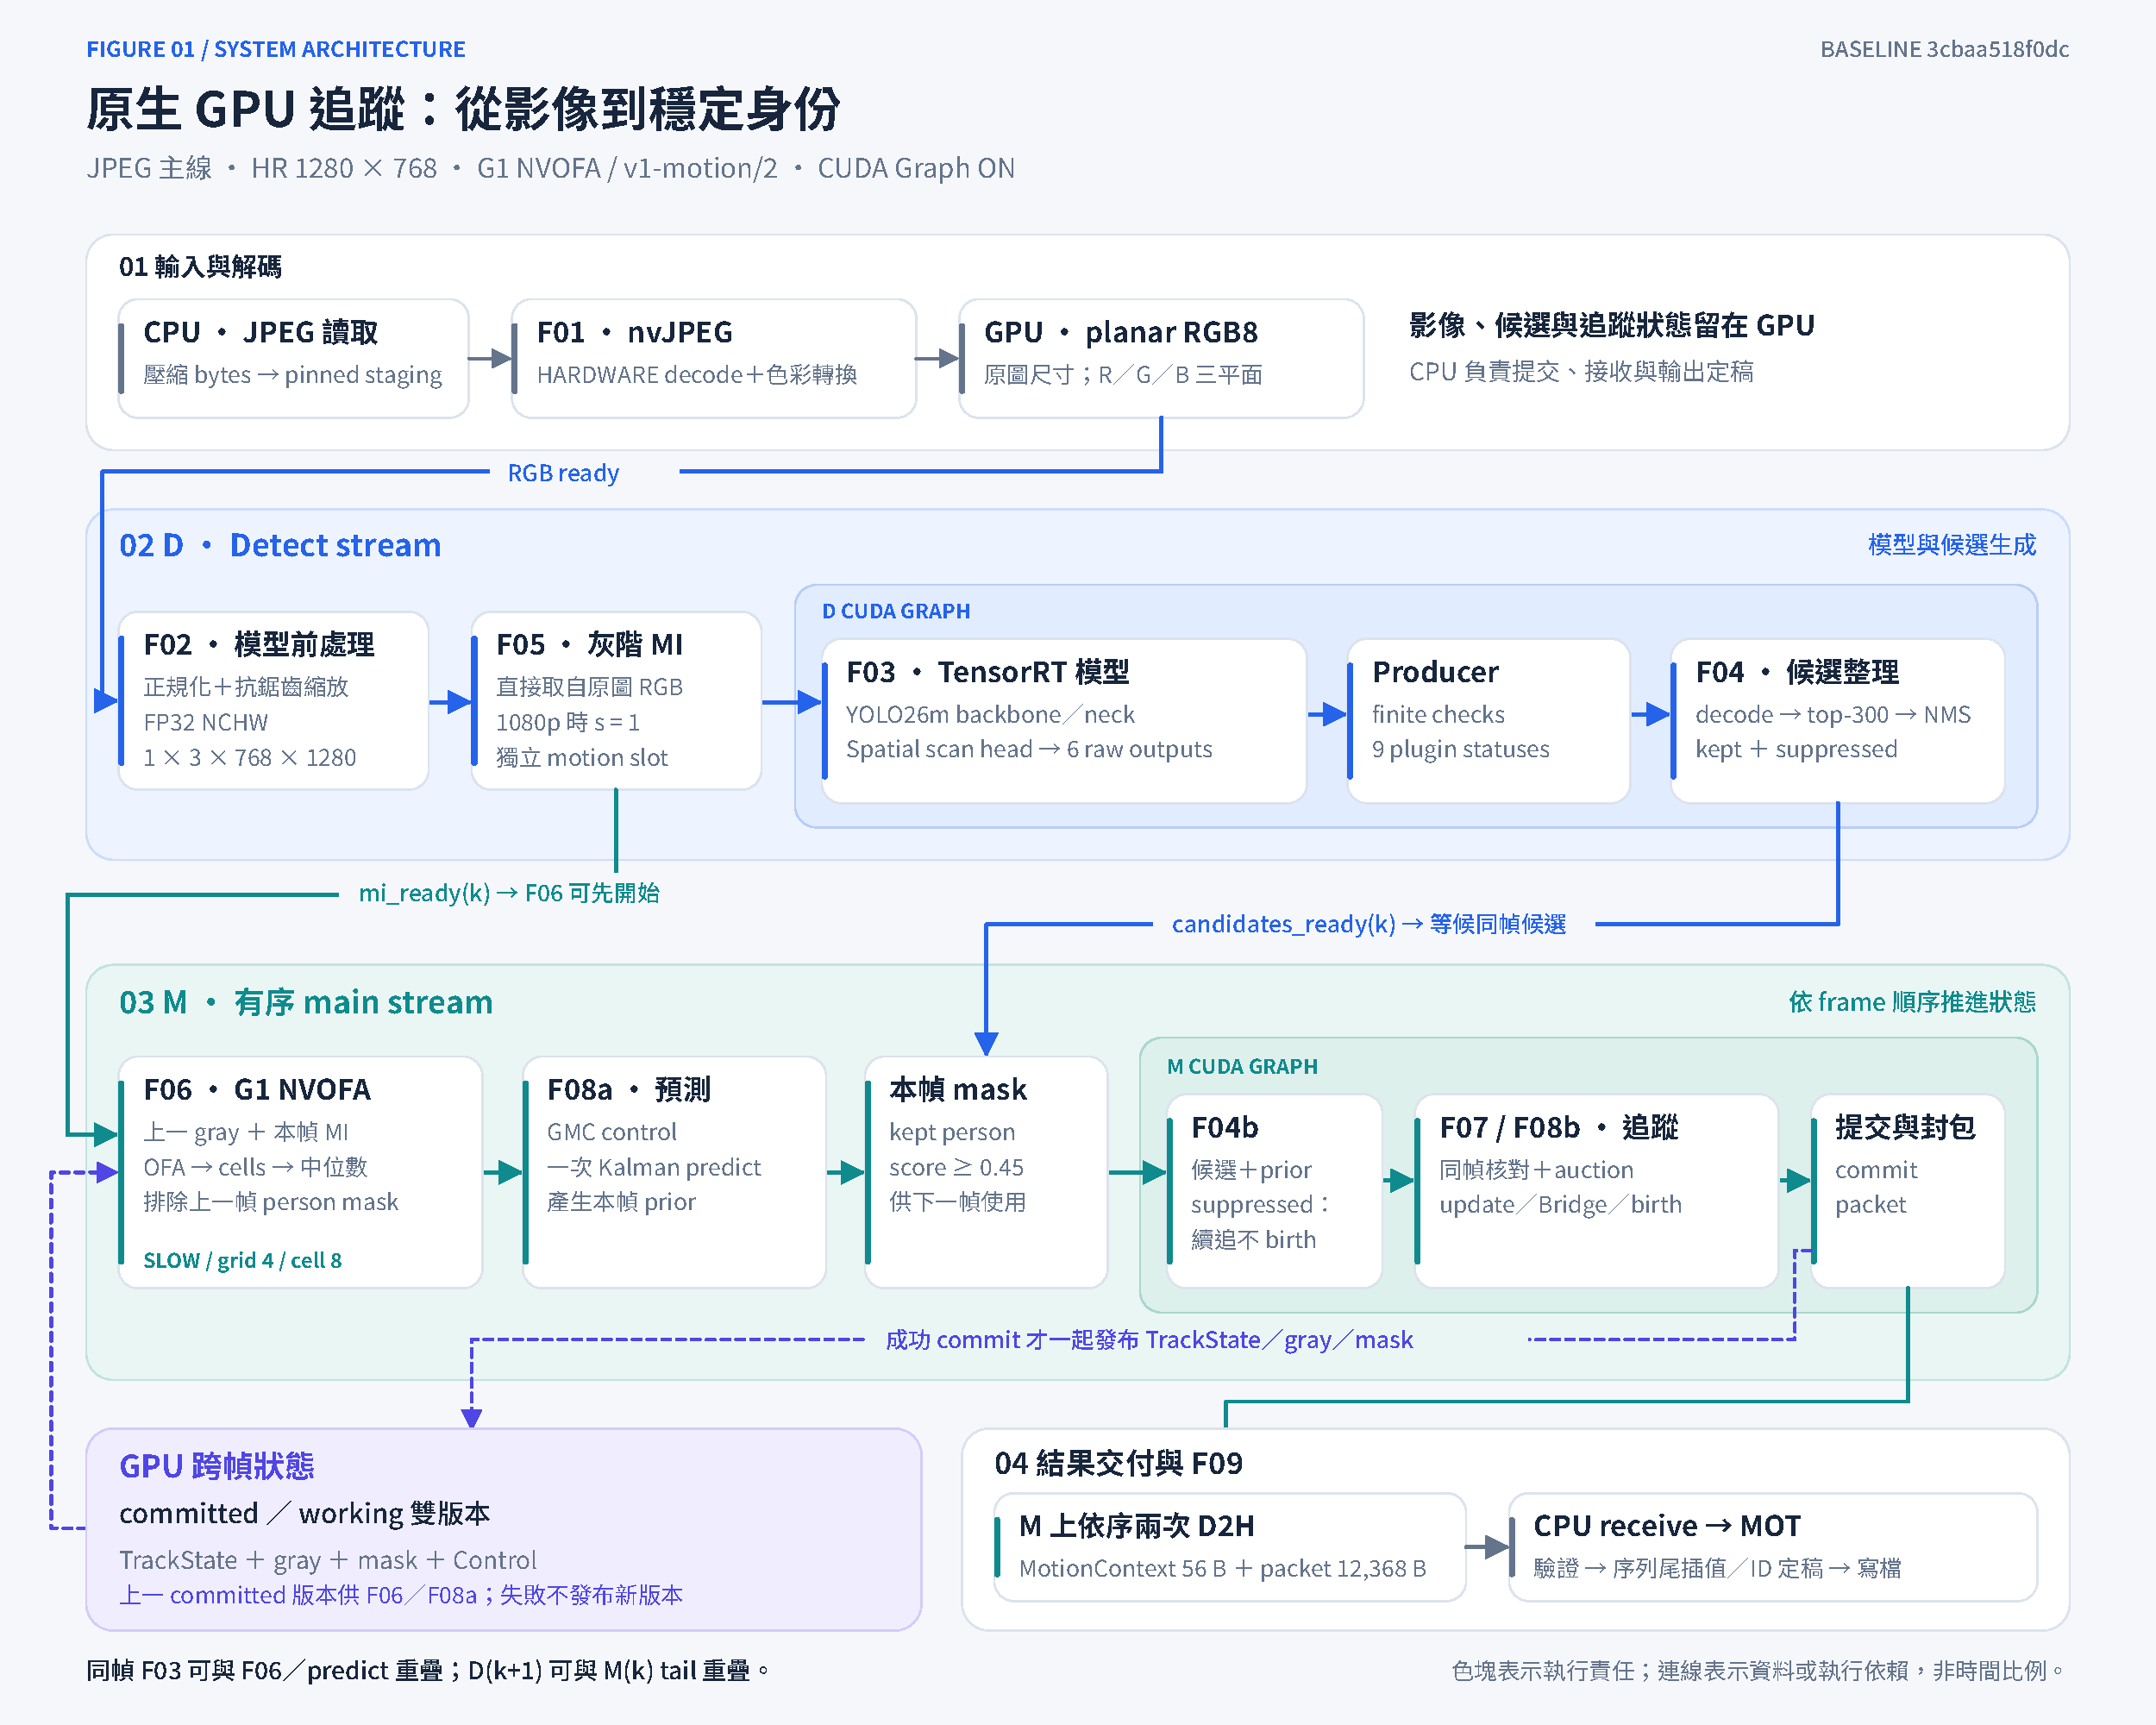
\includegraphics[width=\textwidth]{assets/system.pdf}
\caption{JPEG 主線與資料責任。Graph 標籤表示 capture 範圍；跨 stream 排程與 D2H 仍由 session 管理。}
\label{fig:system}
\end{figure}
\source{\path{src/tracking_session.cpp}、\path{cuda/flow_motion.cu} 及 TRACKING\cite{tracking}。}

\subsection{模型與跨幀狀態}
F03 使用 YOLO26m backbone／neck，P3／P4／P5 各接獨立 spatial scan head，輸出六個 FP32 cls／reg 張量，共 20,160 positions。三尺度 head 先降採樣再執行四方向 Cross-Scan、selective scan 與 merge。這是 \textbf{T=1 spatial 路徑}，每次 scan 從零初始狀態開始；跨幀狀態由 tracking 的 motion、TrackState 與 control 保存，並非 temporal Mamba hidden state。

\begin{figure}[H]
\centering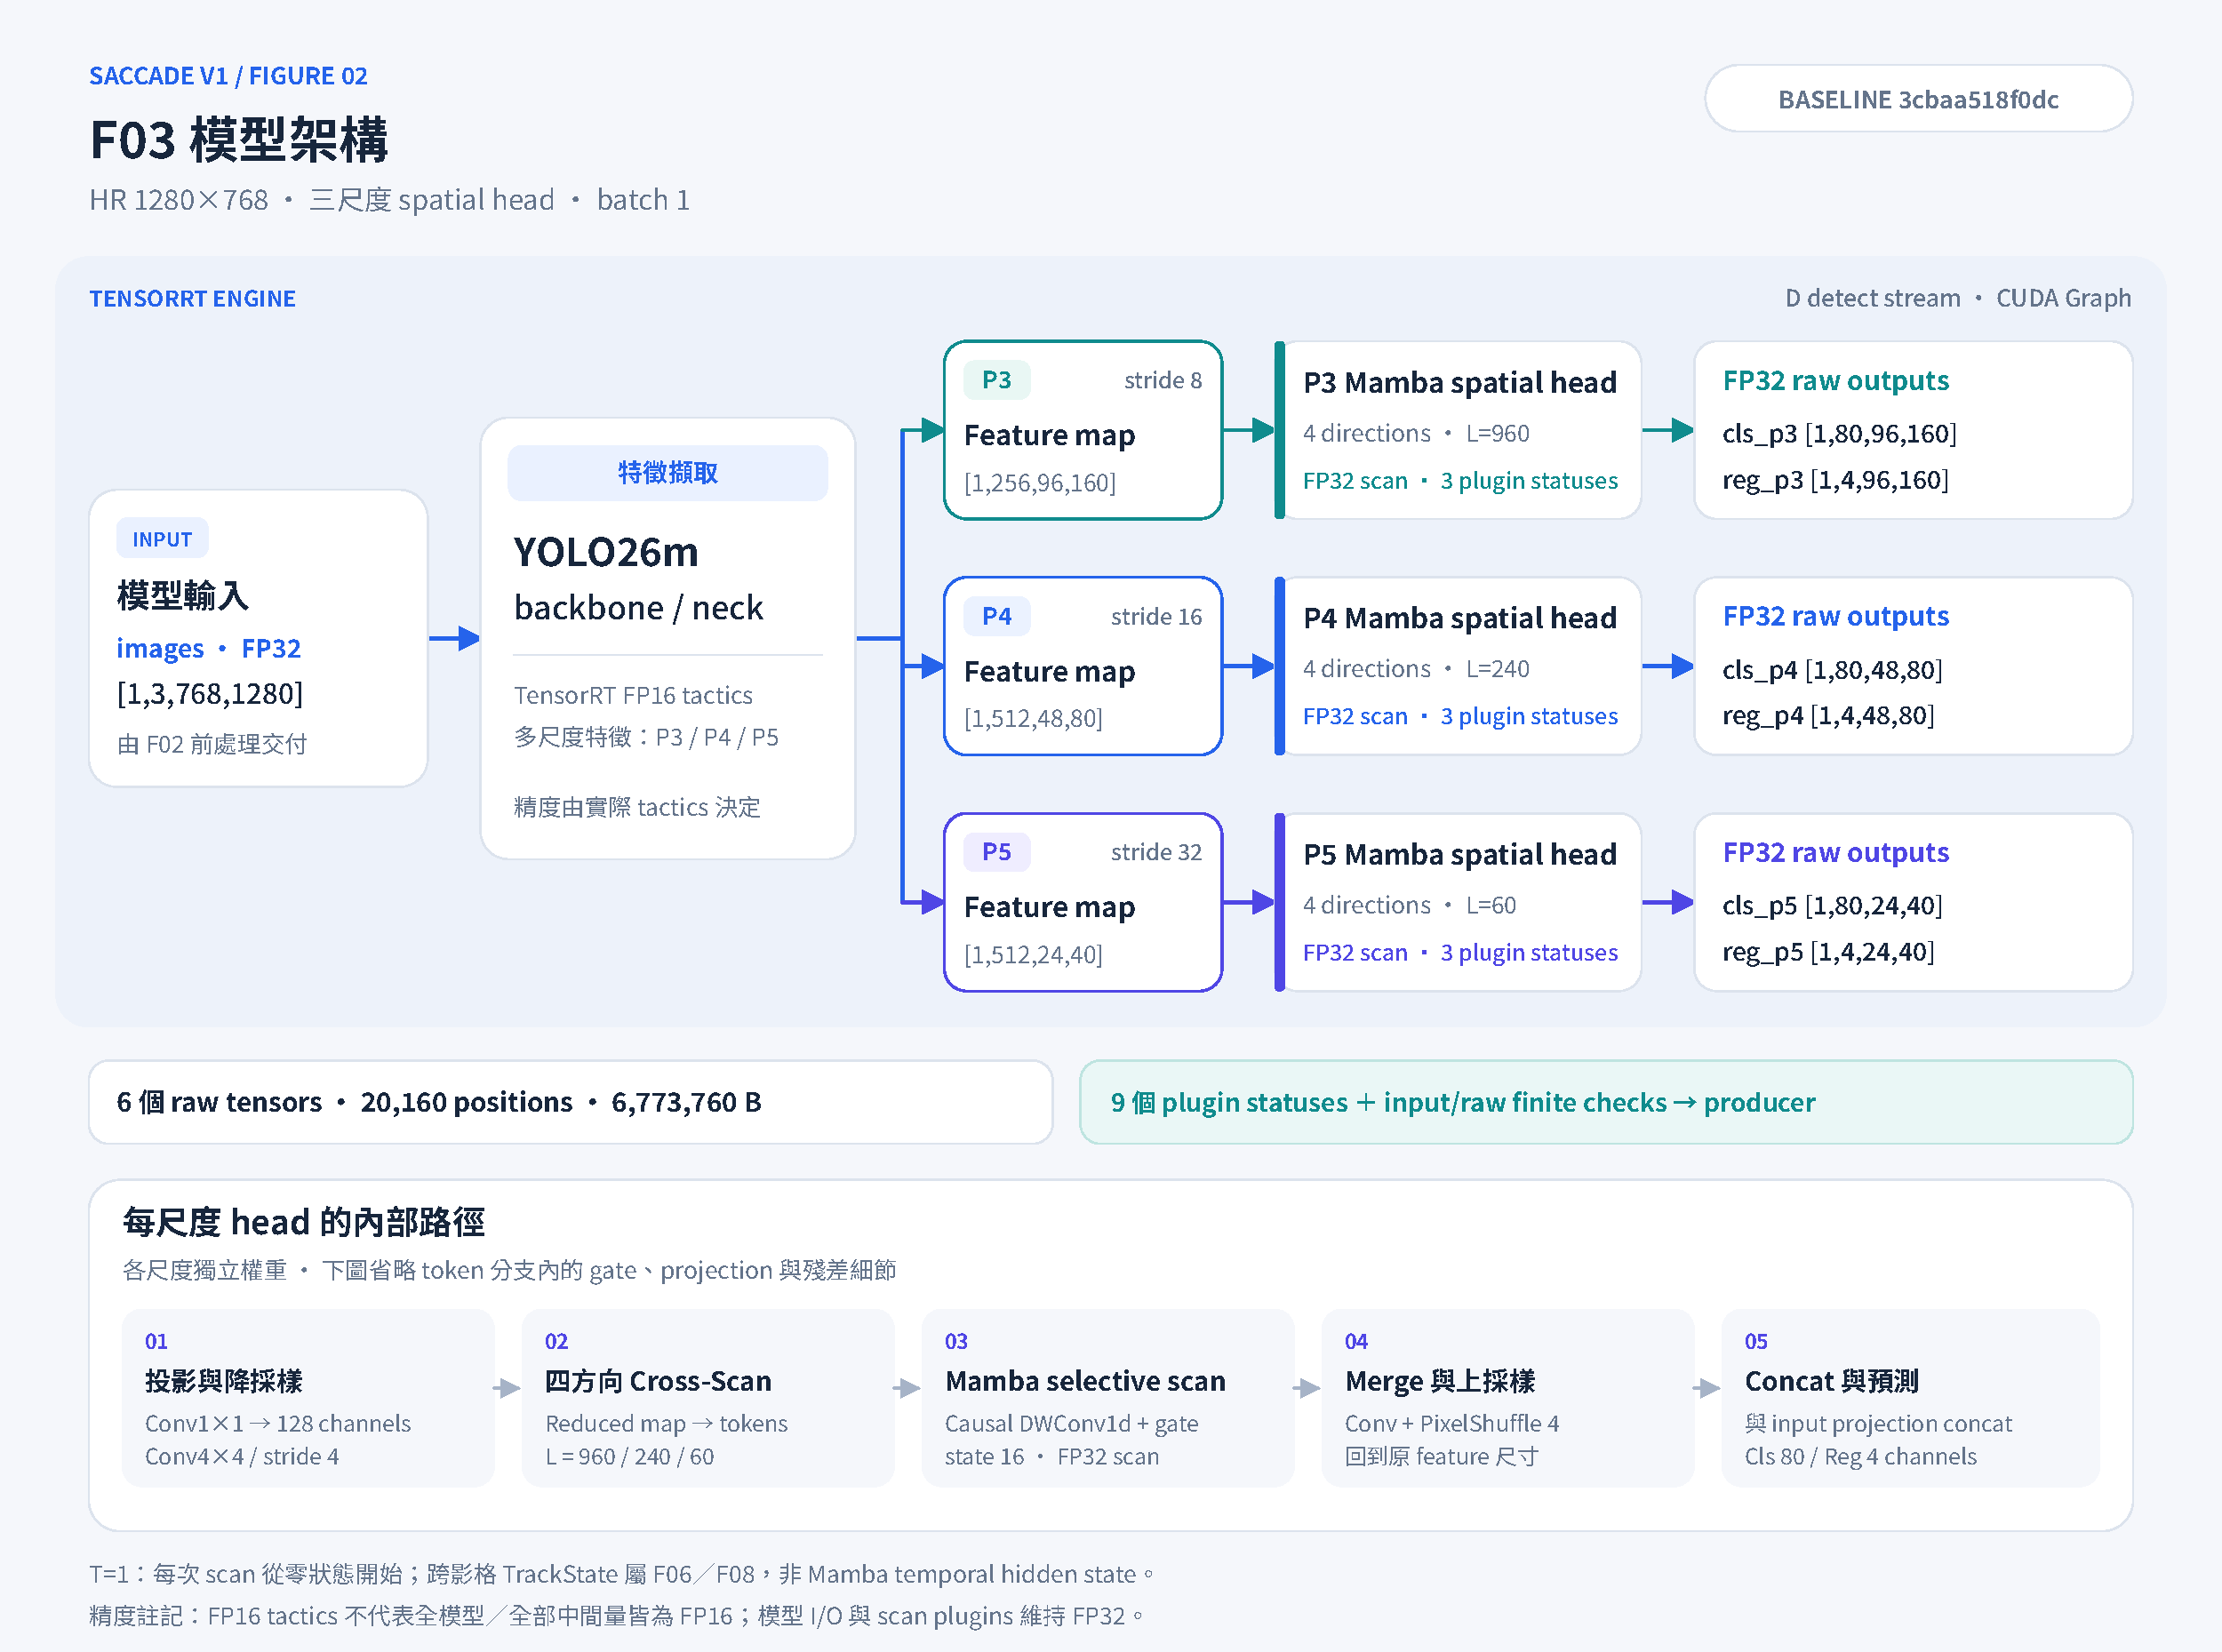
\includegraphics[width=\textwidth]{assets/model.pdf}
\caption{F03 模型資料介面。FP16 tactics 不表示所有張量、scan 與 tracker 都改成 FP16；框內算子未逐層展開。}
\label{fig:model}
\end{figure}

HR input payload 為 11.25 MiB，六個 raw outputs 共約 6.460 MiB。這是 GPU 張量大小，不是每幀 host-device 傳輸量，亦不含 workspace 與中間量。偵測候選先按全類別 top-300 再篩 person；tracker 使用幾何與運動關聯，不使用 ReID。

G1 以原圖 RGB 另產生灰階影像供 NVOFA，排除前次 committed person mask 後作分量中位數歸約。Mask 使用 class 0、score 至少 0.45 的 kept 候選；本幀 mask 供下一 committed frame 使用。早期 DATAFLOW 的 PCR／cuFFT 主圖屬歷史設計，現行 G1 以 TRACKING §20 為準。

\subsection{排程、所有權與背壓}
\begin{figure}[H]
\centering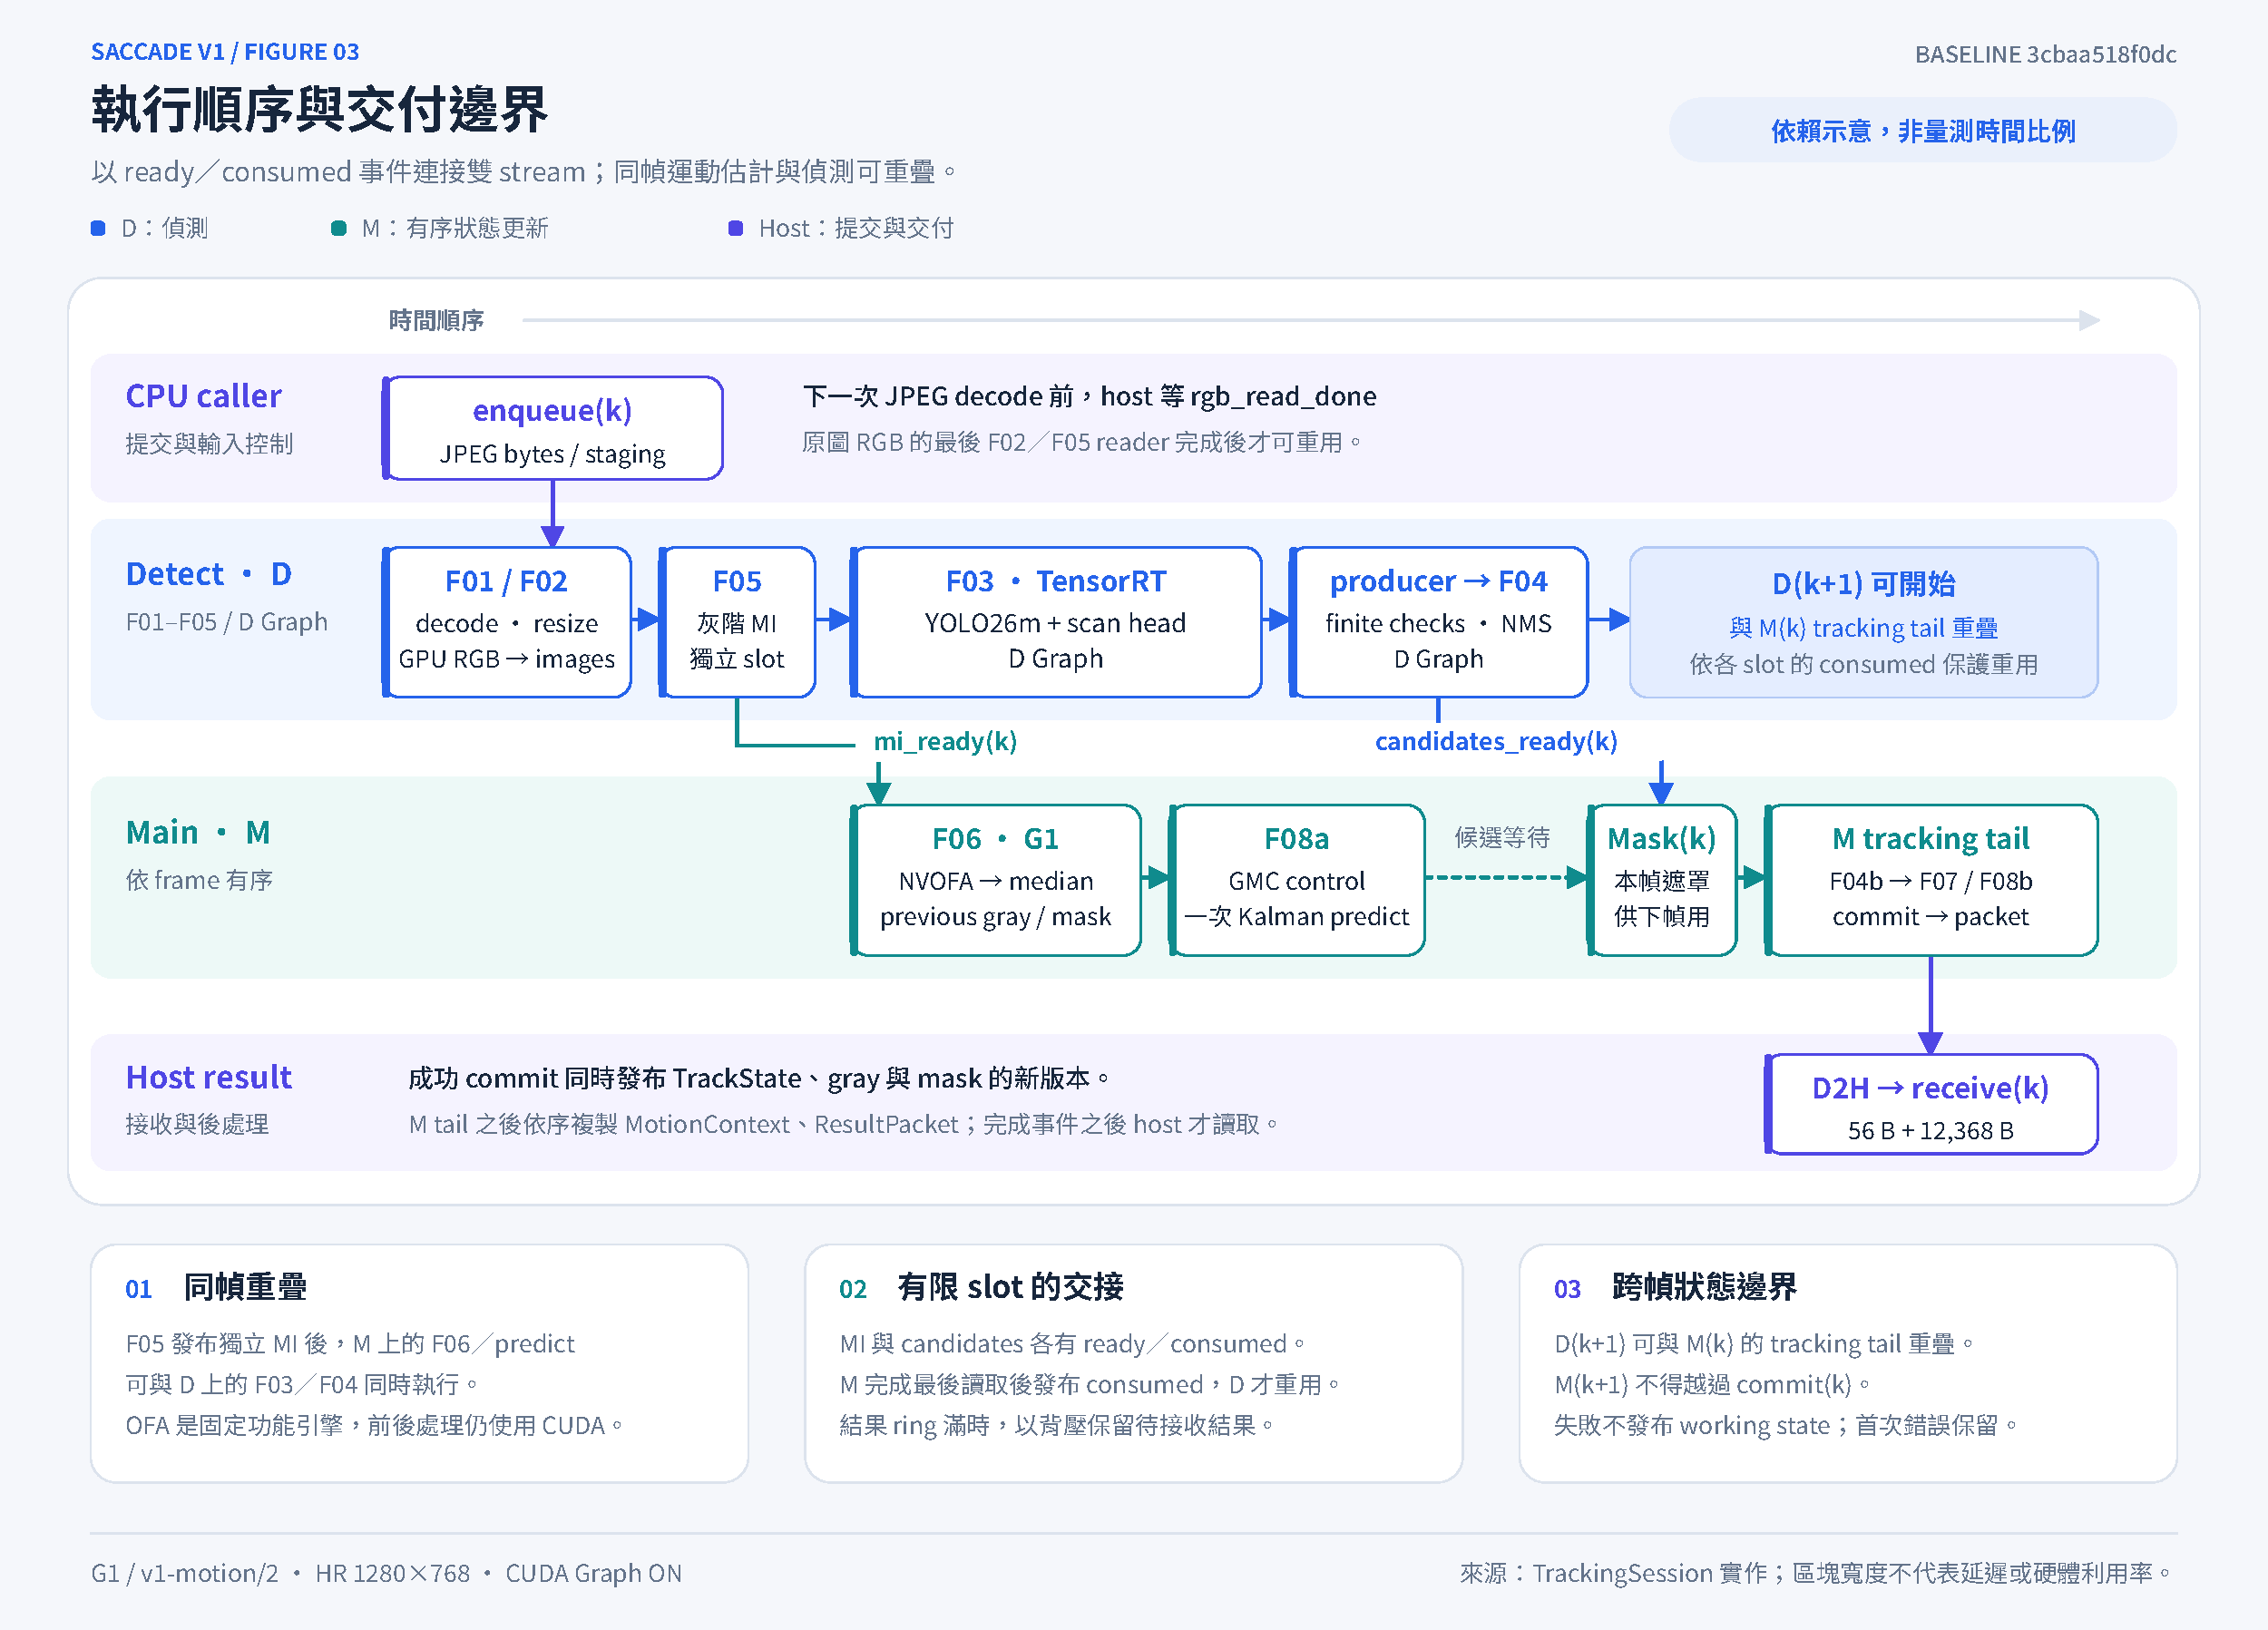
\includegraphics[width=\textwidth]{assets/schedule.pdf}
\caption{D／M 與 host 的必要順序。框寬不表示實測時間；M 的下一幀不得越過前幀 commit。}
\label{fig:schedule}
\end{figure}

\begin{table}[H]
\caption{主要資源的回收條件}
\small
\noindent\begin{tabularx}{\textwidth}{@{}P{33mm}Y@{}}
\toprule
資源 & 可安全重用的條件 \\
\midrule
共用 RGB & 下一次 nvJPEG decode 前，host 等待 F02／F05 最後讀取完成 \\
MI ring & D 在重用 slot 前等 M 的 \code{mi_consumed} \\
Candidate ring & 最後候選讀取完成；預設 Graph 路徑於 M tail 完成後 release \\
Committed／working & 只在成功 commit 後一起發布 TrackState、gray、mask 與 Control \\
模型 input／raw & 同一 D stream 次序及固定地址契約；不能任意借予下一推論 \\
Host result ring & receive 消費前保留 slot；滿時背壓，不覆寫尚未交付結果 \\
\bottomrule
\end{tabularx}
\end{table}

是否使用 Graph、session 的 serial／pipelined 排程，以及 caller 的 single／queued 提交與接收，是三項獨立設定。D(k+1) 可與 M(k) tail 重疊，但重疊會競爭資源，並不保證每階段時間都縮短。

\subsection{影片／串流入口}
\code{track_stream} 預設為 FFmpeg 收流／demux、NVDEC 解碼、device NV12／P010、CUDA 色彩轉換及同一 TrackingSession。CPU decode 須顯式選定，GPU 失敗不自動切 CPU。CLI 逐幀 enqueue 後立即 receive／flush，result ring=1，沒有多幀 queued 的吞吐主張。

串流使用 \code{stream-observations/1}，不作序列尾插值與全序列 ID 重編號；JPEG sequence 的 \code{v1-mot/1} 則在 EOF 後定稿。因此，離線 MOT 的完整輸出不能直接當作即時輸出的相同行為承諾。來源 PTS 也未改變固定步長 Kalman dt。

\section{交付內容與重現方式}
本次交付包含可編譯的 LaTeX 原稿、PDF、三張向量圖、建置說明、本次量測收據及既有三模型比較摘要。原專案的正式證書、歷史 FAIL／OPEN 與 source custody 保持原樣。報告編製與補測未變更 runtime 預設或模型；本次修訂只讀取既有比較結果，未執行訓練、品質重評或新的 sanitizer gate。

\noindent\begin{tabularx}{\textwidth}{@{}P{36mm}Y@{}}
\toprule
交付項目 & 專案相對路徑 \\
\midrule
正式報告／原稿 & \path{docs/reports/latex/report1/report.pdf}、\path{report.tex} \\
圖稿 & 同目錄 \path{assets/}；原 SVG 在 \path{docs/reports/assets/report1-3cbaa518f0dc/} \\
重建說明 & 同目錄 \path{README.md}、\path{Makefile} \\
本次逐幀補測 & \path{evidence/report1/2026-11-11-g1-live/} \\
本次完整離線 & \path{evidence/report1/2026-11-11-g1-offline-e2e/} \\
三模型／跨資料集 & \path{evidence/model-comparison/2026-11-11-yolo26m-primary156/bundle/}；同目錄 \path{model-comparison.tex}、\path{comparison-sources.json} \\
歷史重算 & \path{evidence/report1/2026-11-11-detailed-report/latency-summary.json} \\
版本收尾 & \path{docs/history/2026-11-11-first-report-baseline.md} \\
目前狀態 & \path{docs/STATUS.md}、\path{docs/BACKLOG.md} \\
\bottomrule
\end{tabularx}

正式報告可於其目錄執行 \code{make} 以 XeLaTeX 重建。固定程式與歷史證據可用 \code{git show <完整 SHA>:<path>} 取得。相對連結在日後 checkout 中可能顯示新內容，長期引用應同時保留 commit、路徑及 hash。可選功能若要改為預設，須另做部署驗收。

\appendix
\clearpage
\section{計時定義與詳細量測條件}
\begin{longtable}{@{}P{31mm}P{51mm}P{74mm}@{}}
\caption{效能指標的邊界與限制}\label{tab:timing}\\
\toprule 指標 & 起點與終點 & 包含與排除 \\
\midrule\endfirsthead
\toprule 指標 & 起點與終點 & 包含與排除 \\
\midrule\endhead
Single latency & enqueue 前至同幀 blocking receive 返回 & JPEG 預載；無前幀在途。含 host 提交至封包返回，不含磁碟、constructor、暖機與寫檔 \\
Queued delivery & enqueue 前至 caller 實際 receive 該幀 & 含在途等待、資源競爭與 caller 延後取回；不等於 GPU 完成時間 \\
Queued interval & 整段 wall time 除以完成幀數 & 描述 pipeline 吞吐，不代表任何個別幀的交付延遲 \\
Sequence ms/frame & 首張 JPEG 讀取前至 finish／drain 完成後除以幀數 & 含讀檔、lazy capture、output.add；不含 constructor、checked close、尾端插值與最終檔案寫入 \\
GPU busy & 每階段同幀活動區間的聯集 & 不含區間間隙；不能與重疊階段直接相加 \\
GPU envelope & 第一個活動開始至最後活動結束 & 含空檔與等待；CUDA event、host clock 與 profiler 數值不同 \\
外部即時 E2E & 相機曝光／可信時間戳至實際消費端 & 應涵蓋網路、demux、decode reorder、GPU、背壓與輸出；本次未量測 \\
\bottomrule
\end{longtable}

Clean-source ABBA 使用 MOT17-10 前 140 幀，每 fresh session 從 frame 0 建立相同歷史，20 幀暖機、120 幀量測，JPEG 預載、Graph ON、result ring=4。兩輪 A\ensuremath{\to}B\ensuremath{\to}B\ensuremath{\to}A 共 32 sessions，每 backend 有 960 個 single 樣本與 8 個 queued intervals。分位數從全部逐幀樣本計算，沒有平均各 run 的 p95，也沒有刪除長尾。此處的 A／B 為歷史 \code{v1-motion/1} 兩版本，與本次補測分開。

G1 舊正式驗收 serial 只有各序列 wall time 與平均值，缺少逐幀樣本，故不能補造其 p95／p99。G1 Nsight 的 30 幀中，29 幀執行 OFA，28 幀的可觀測外包界限完全落在 F03 內；中位界限約 2.22 ms。這是輸入 copy 完成到 cells 開始的間接界限，工具未直接看到 OFA 固定功能引擎本體，不可稱精確 engine 延遲。

\section{歷史分序列與受控加速結果}
\begin{table}[H]
\caption{G1 正式驗收七序列吞吐，\code{fae5cb7}／\code{v1-motion/2}}
\small
\noindent\begin{tabularx}{\textwidth}{@{}Yrrrr@{}}
\toprule
序列 & 幀數 & Serial ms/frame & Pipeline ms/frame & Pipeline FPS \\
\midrule
MOT17-02-SDP & 600 & 6.916350 & 5.263333 & 190.0 \\
MOT17-04-SDP & 1,050 & 7.158781 & 5.572737 & 179.4 \\
MOT17-05-SDP & 837 & 6.176643 & 5.314190 & 188.2 \\
MOT17-09-SDP & 525 & 6.694933 & 5.341175 & 187.2 \\
MOT17-10-SDP & 654 & 6.862462 & 5.566458 & 179.6 \\
MOT17-11-SDP & 900 & 6.872489 & 5.488419 & 182.2 \\
MOT17-13-SDP & 750 & 6.957507 & 5.460227 & 183.1 \\
\midrule
加權／總計 & 5,316 & 6.817652 & 5.443318 & 183.711 \\
\bottomrule
\end{tabularx}
\end{table}
Serial 為 36,242.64 ms／5,316 幀；pipeline 每序列三次，每臂共 15,948 幀。G1 相對舊 PCR 的總時間增加 2.69853\%，通過當時總計 3\% 上限；個別序列並非全部低於 3\%。測試每組 PCR 先、G1 後，未反轉順序，不推導為普遍固定差值。\cite{g1}

\begin{table}[H]
\caption{Clean-source ABBA 詳細結果：舊 \code{v1-motion/1}}
\small
\noindent\begin{tabularx}{\textwidth}{@{}Yrrr@{}}
\toprule
指標 & 加速前 & 加速後 & 變化 \\
\midrule
F02 isolated Graph（µs） & 147.138 & 88.483 & −39.86\% \\
完整 F03 Graph（ms） & 5.241696 & 4.904589 & −6.43\% \\
Single mean（ms） & 7.092724 & 6.626377 & −6.58\% \\
Single p50（ms） & 7.045901 & 6.568929 & −6.77\% \\
Single p95（ms） & 7.524795 & 7.059455 & −6.18\% \\
Single p99（ms） & 7.719933 & 7.312254 & −5.28\% \\
Single min（ms） & 6.589859 & 6.209250 & 僅記錄 \\
Single max（ms） & 8.385982 & 8.595218 & 僅記錄 \\
Queued interval（ms/frame） & 5.536401 & 5.123390 & −7.46\% \\
Queued FPS & 180.623 & 195.183 & +8.06\% \\
\bottomrule
\end{tabularx}
\end{table}

F02 的約 40\% primitive 改善，與 F02／F03 合併後 single 約 6.6\% 改善是不同範圍。歷史 F03 分析中 backbone／neck 占 kernel duration 加總 66.12\%，conv／GEMM 占 63.73\%，scan core 占 15.63\%；這些比例為模型內部歸因，不是整條端到端延遲比例。\cite{abba,backbone}

歷史 cuFFT 的單次 ring depth probe 中，depth 1／2／4 的 delivery mean 為 6.993／10.740／21.289 ms，interval 為 7.002／5.396／5.401 ms/frame。depth 2 的吞吐接近 depth 4 且交付較快，但該輪沒有 ABBA 或 G1 重驗，不據此更改現行四格預設。\cite{resource}

\clearpage
\begin{thebibliography}{99}
\addcontentsline{toc}{section}{證據與參考文件}
\footnotesize
\setlength{\itemsep}{0.1em}
\linespread{1.08}\selectfont
\bibitem{closeout} Saccade v1，第一輪報告版本收尾，2026-11-11。\newline\path{docs/history/2026-11-11-first-report-baseline.md}；\path{evidence/report1/2026-11-11-closeout/checks.json}。
\bibitem{status} Saccade v1，目前狀態與文件入口，報告基準內版本。\newline\path{docs/STATUS.md}。
\bibitem{m4} M4 正式評估與 P01 收尾，2026-11-03，\code{cad5298}。\newline\path{evidence/m4/2026-11-03-formal-cad5298/REPORT.md}。
\bibitem{g1} G1／\code{v1-motion/2} TrackingSession 驗收，2026-11-05，\code{fae5cb7}。\newline\path{evidence/tracking-session/2026-11-05-v1-motion-2-acceptance-2/REPORT.md}；其 \path{capture/throughput-runs.csv}、\path{serial-latency.csv}、\path{ofa-overlap.csv}。
\bibitem{f02correct} F02／F03 clean-source 整合補驗，2026-11-05，\code{23ade53}。\newline\path{evidence/f02-f03/2026-11-05-clean-23ade53/REPORT.md}。
\bibitem{abba} F02／F03 clean-source ABBA 效能補驗，2026-11-05。\newline\path{evidence/f02-f03/2026-11-05-clean-performance/REPORT.md}、\path{analysis.json}、\path{tracking-latencies.csv}、\path{tracking-runs.csv}。
\bibitem{nsa} NSA v2／量測框正式驗收，2026-11-09，\code{527ffe5}。\newline\path{evidence/nsa-v2/2026-11-09-formal-527ffe5/REPORT.md}、\path{SUMMARY.json}。
\bibitem{p08} P08 設定與事件工具及開發來源證據，2026-11-06。\newline\path{docs/P08_TOOLS.md}；\path{evidence/p08/2026-11-06-development/REPORT.md}。
\bibitem{tracking} Tracking 規格、G1 現行契約與程式。\newline\path{docs/TRACKING.md} §20；\path{src/tracking_session.cpp}；\path{cuda/flow_motion.cu}；\path{include/saccade/model_profile.hpp}。
\bibitem{stream} 即時串流與 NVDEC 開發驗證，2026-11-05。\newline\path{docs/STREAMING.md}；\path{evidence/streaming/2026-11-05-development/REPORT.md}。
\bibitem{backlog} 尚未完成項目與適用界線，報告基準內版本。\newline\path{docs/BACKLOG.md}；\path{docs/PREPROCESS_USAGE_POLICY.md}。
\bibitem{hrsan} HR 完整路徑 sanitizer 補驗，2026-11-05。\newline\path{evidence/hr-sanitizer/2026-11-05-a00ab3a/REPORT.md}。
\bibitem{bounded} HR 有界排隊 sanitizer 補驗，2026-11-06。\newline\path{evidence/hr-sanitizer/2026-11-06-bounded-queue/REPORT.md}。
\bibitem{backbone} F03 backbone／head 瓶頸分析，2026-11-04，開發來源。\newline\path{evidence/f03-backbone-head/2026-11-04/REPORT.md}。
\bibitem{resource} 硬體資源與排程報告，2026-11-04，\code{865bb10}＋dirty。\newline\path{evidence/resource-schedule/2026-11-04/REPORT.md}；\path{raw/queue-depth-summary.json}；\path{stages/stage_summary.csv}。
\bibitem{offline} 本次完整離線端到端補測，2026-11-11。\newline\path{evidence/report1/2026-11-11-g1-offline-e2e/}。計時涵蓋程序啟動至正常退出；不等於逐幀交付延遲或相機端到端。
\bibitem{live} 本次 G1 逐幀延遲補測，2026-11-11。\newline\path{evidence/report1/2026-11-11-g1-live/}。來源、方法、原始樣本、環境與封包比對以該目錄收據為準。
\bibitem{primary156} 官方／微調 YOLO26m 與現行 HR Mamba：primary156 TensorRT 品質研究，2026-11-11。\newline\path{evidence/model-comparison/2026-11-11-yolo26m-primary156/bundle/REPORT.md}；\path{metrics/summary.json}、\path{metrics/per-sequence.csv}、\path{audits/scoring-audit.json}、\path{training-provenance.json}、\path{evaluation-scope.json}。156 段已曝露，非 blind test 或正式部署驗收。
\bibitem{trtcompare} TensorRT 三方性能與品質比較，2026-11-11。\newline\path{evidence/model-comparison/2026-11-11-yolo26m-trt-performance/REPORT.md}；\path{performance/model/summary.json}、\path{performance/pipeline/summary.json}、\path{model-memory.json}、\path{validation.json}。保留 FP16 數值 screen FAIL 與原始量測邊界。
\end{thebibliography}
\end{document}
